\documentclass[a4paper,11pt]{article}

\usepackage[utf8]{inputenc}
\usepackage[top=2cm, left = 2cm , right=2cm , bottom=2cm]{geometry}
\usepackage{amsmath}
\usepackage{graphicx}
\usepackage{float}
\usepackage{listings}
\usepackage[brazil]{babel}

\usepackage{color}

\definecolor{mygreen}{rgb}{0,0.6,0}
\definecolor{mygray}{rgb}{0.5,0.5,0.5}
\definecolor{mymauve}{rgb}{0.58,0,0.82}

\lstset{
  backgroundcolor=\color{white},   % choose the background color; you must add
                                   % \usepackage{color} or \usepackage{xcolor};
                                   % should come as last argument
  basicstyle=\footnotesize,        % the size of the fonts
  breakatwhitespace=false,         % sets if automatic breaks should only happen
                                   % at whitespace
  breaklines=true,                 % sets automatic line breaking
  captionpos=b,                    % sets the caption-position to bottom
  commentstyle=\color{mygreen},    % comment style
  escapeinside={\%*}{*)},          % if you want to add LaTeX within your code
  extendedchars=true,              % lets you use non-ASCII characters; for
                                   % 8-bits encodings only, does not work with
                                   % UTF-8
  frame=single,	                 % adds a frame around the code
  keepspaces=true,                 % keeps spaces in text, useful for keeping
                                   % indentation of code (possibly needs
                                   % columns=flexible)
  keywordstyle=\color{blue},       % keyword style
  language=Matlab,                 % the language of the code
  numbers=left,                    % where to put the line-numbers; possible
                                   % values are (none, left, right)
  numbersep=5pt,                   % how far the line-numbers are from the code
  numberstyle=\tiny\color{mygray}, % the style that is used for the line-numbers
  rulecolor=\color{black},         % if not set, the frame-color may be changed
                                   % on line-breaks within not-black text
                                   % (e.g. comments (green here))
  showspaces=false,                % show spaces everywhere adding particular
                                   % underscores; it overrides
                                   % 'showstringspaces'
  showstringspaces=false,          % underline spaces within strings only
  showtabs=false,                  % show tabs within strings adding particular
                                   % underscores
  stepnumber=2,                    % the step between two line-numbers. If it's
                                   % 1, each line will be numbered
  stringstyle=\color{mymauve},     % string literal style
  tabsize=2,                       % sets default tabsize to 2 spaces
  title=\lstname                   % show the filename of files included with
                                   % \lstinputlisting; also try caption instead
                                   % of title
}

\pagestyle{plain}

\graphicspath{{./Imagens/}}

\begin{document}

\begin{center}
\textbf{Experiência 2} \\
\hspace{5pt}
Prof. Marconi Kolm Madrid \\
EA722 - 2017/2
\end{center}

\begin{center}
Danilo Pereira Titato - RA 122541 \\
Giovani Granzotto Oliani - RA 146253 \\
Pedro Gabriel Calixto Mendonça - RA 118363 \\
\end{center}

\textbf{1 - 5.}
Malha aberta com mola de dureza média ($338.6 N/m$) e ganho do pré-filtro como
calculado no Experimento 1 ($k_{pf} = 0.0230$):

\begin{figure}[H]
\centering
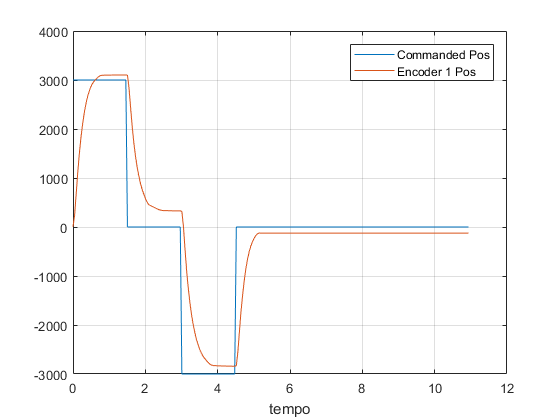
\includegraphics{exp02e05}
\caption{Resposta em malha aberta, mola de dureza média}
\end{figure}

\hspace{5pt}

\textbf{6.}
Malha fechada com mola de mola de dureza média ($338.6 N/m$) e ganhos do
pré-filtro como calculados no Experimento 1 para cada $k_p$ usado
($0.03$, $0.12$, $0.24$):

\begin{figure}[H]
\centering
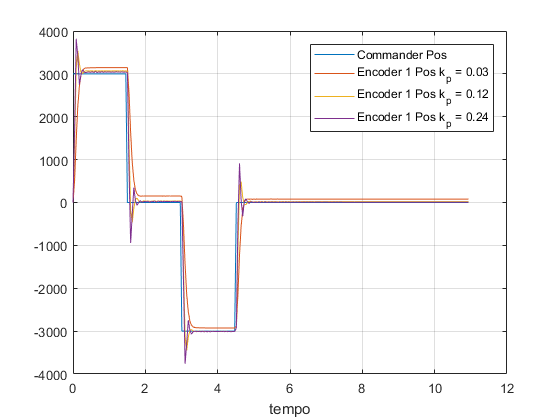
\includegraphics{exp02e06}
\caption{Resposta em malha fechada, mola de dureza média}
\end{figure}
\begin{figure}[H]
\centering
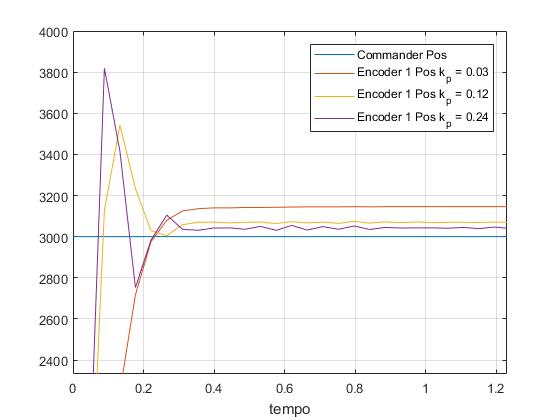
\includegraphics{exp02e06-zoom}
\caption{Resposta em malha fechada, gráfico ampliado}
\end{figure}
\begin{figure}[H]
\centering
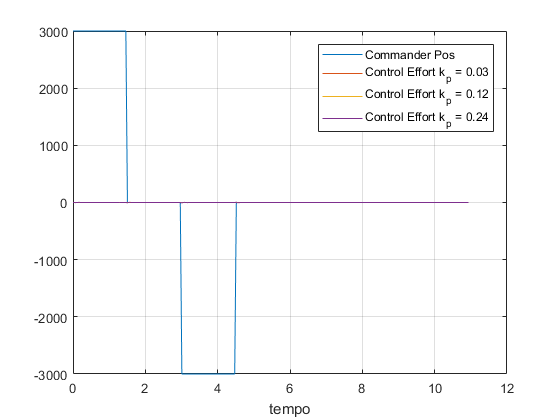
\includegraphics{exp02e06-control-effort}
\caption{Control Effort em malha fechada}
\end{figure}

\textbf{7.}
\begin{figure}[H]
\centering
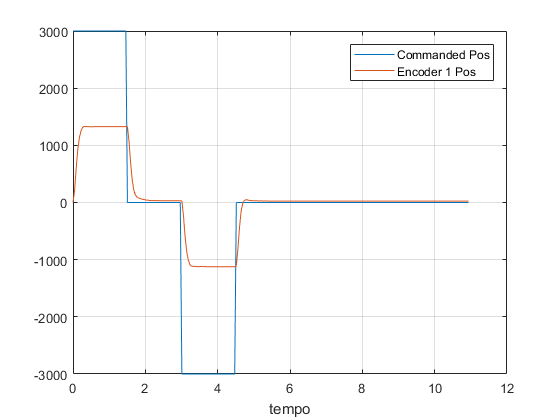
\includegraphics{exp02e07-aberta}
\caption{Resposta em malha aberta, mola de maior dureza}
\end{figure}
\begin{figure}[H]
\centering
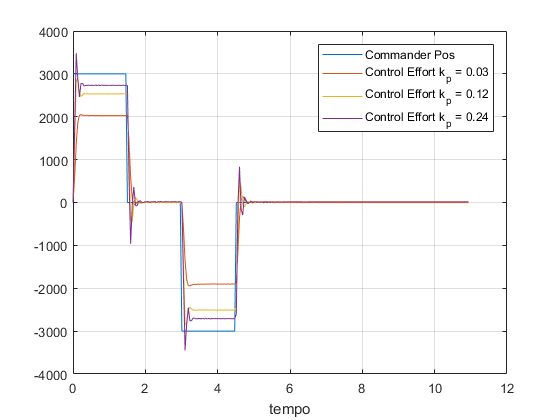
\includegraphics{exp02e07-fechada}
\caption{Resposta em malha fechada, mola de maior dureza}
\end{figure}
\begin{figure}[H]
\centering
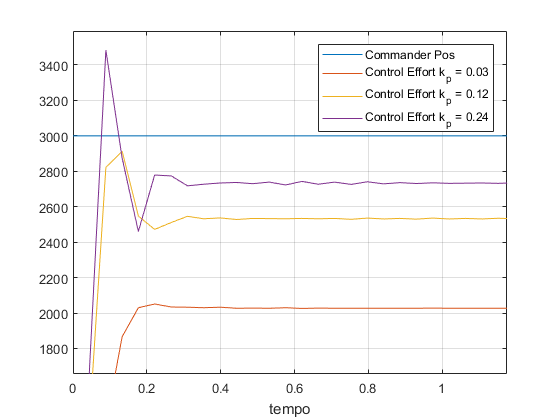
\includegraphics{exp02e07-fechada-zoom}
\caption{Resposta em malha fechada, gráfico ampliado}
\end{figure}

\hspace{5pt}

\textbf{8. (a)}
Relevando distúrbios e erro experimental, as respostas do
sistema de malha fechada coincidem com as esperadas teoricamente, como visto nos
gráficos resultados do Experimento 1.

Comparado com o sistema de malha fechada, o sistema de malha aberta possui um
controle maior, fazendo com que a resposta tenha um tempo de subida menor e se
estabilize mais rapidamente.
No regime permanente, o erro de regime do sistema de malha aberta é menor do que
o erro do sistema de malha fechada com $k_p = 0.03$. Porém, à medida que o $k_p$
aumenta, esse erro vai sendo diminuído. \\

\textbf{(b)}
Conforme $k_p$ é aumentado, vê-se que o valor do pico de \textit{overshoot}
aumenta. É possível observar também que a quantidade de oscilação aumenta,
ocorrendo três cruzamentos com o zero para o maior valor de $k_p$ antes da
estabilização, enquanto para o menor valor de $k_p$ não há oscilação após a
queda do \textit{overshoot}.

Quanto ao erro, ao contrário do sistema de malha aberta quando perturbado, esse
consegue ser regulado quando se trata do sistema de malha fechada. À medida que
o $k_p$ aumenta, o valor de regime da resposta aumenta. Desse modo, mesmo
havendo um distúrbio no parâmetro (neste caso, a constante elástica da mola), é
possível regular-se o erro de regime através do ganho $k_p$ do controlador
proporcional.

\end{document}